\chapter{Satellite Design}
\label{chap:SatDesign}
To simulate the ADCS of the satellite the sensors and actuators that will be used for the CubeSat must be decided. This decision is based on the current trend and implementation of CubeSat as well as what is required of this mission of pointing the payload towards the Earth during eclipse and being sun-following otherwise.

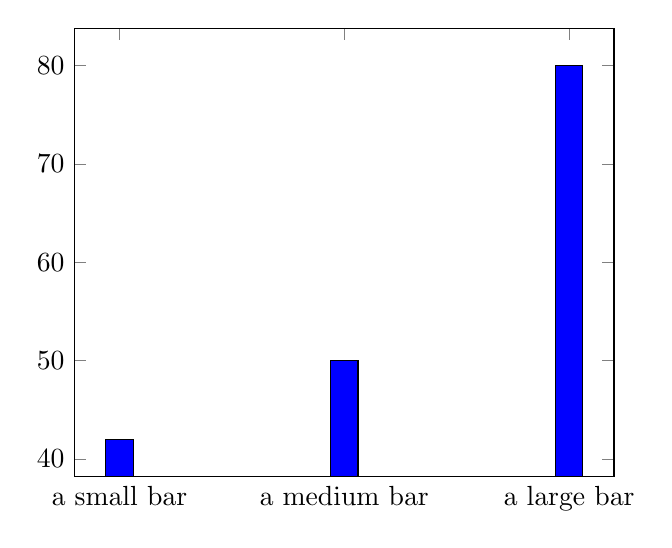
\begin{tikzpicture}
\begin{axis}[
symbolic x coords={a small bar,a medium bar,a large bar},
xtick=data]
\addplot[ybar,fill=blue] coordinates {
	(a small bar,42)
	(a medium bar,50)
	(a large bar,80)
};
\end{axis}
\end{tikzpicture}

\section{CubeSat}
\textbf{TODO: Inertia, size and other parameters}.

\begin{figure}[h!t!b]
	\centering
	\def\svgwidth{14cm}
	\import{Figures/}{CubeSatDesign.pdf_tex}
	\caption{The modelled satellite, with solar panels.}
	\label{fig:CubeSatDesign}
\end{figure}

\section{Actuators}
\textbf{TODO: Ud and Us and other parameters as well as reaction wheel orientation and inertia}.

\section{Sensors}
\textbf{TODO: The sensors that is implemented as well as the noise variation on each sensor and the placement thereof}.